\documentclass{beamer}

\usepackage{amsmath}
\usepackage{gensymb}

\def\inputGnumericTable{}

\usepackage[latin1]{inputenc}
\usepackage{color}
\usepackage{array}
\usepackage{longtable}
\usepackage{calc}
\usepackage{multirow}
\usepackage{hhline}
\usepackage{ifthen}

\usepackage{lscape}

\usetheme{CambridgeUS}

\title{Assignment 9}
\author{Archit Ganvir (CS21BTECH11005)}
\date{\today}
\logo{\large \LaTeX{}}

\begin{document}
\providecommand{\brak}[1]{\ensuremath{\left(#1\right)}}
\begin{frame}

\titlepage

\begin{abstract}
This document gives the solution for Assignment 9 (Papoulis ch.15 Example 15-9).
\end{abstract}

\end{frame}

\logo{}

\begin{frame}

(Example 15-9) Here the two end-boundary states $e_0$ and $e_{N - 1}$ loop together to form a circle so that $e_{N - 1}$ has neighbors $e_0$ and $e_{N - 1}$ (Fig. 15-3). The random walk continues on this circular boundary by passing from one state either to the right or left neighbor and this corresponds to the following $N \times N$ transition matrix
\begin{align}
P = 
\begin{pmatrix}
0 & p & 0 & 0 & . & . & . & 0 & q \\
q & 0 & p & 0 & . & . & . & . & 0 \\
0 & q & 0 & p & 0 & . & . & . & 0 \\
. & & & & & & & & . \\
. & & & & & & & & . \\
. & & & & & & & & . \\
0 & 0 & . & . & . & . & q & 0 & p \\
p & 0 & . & . & . & . & 0 & q & 0 \\
\end{pmatrix}
\end{align}

\end{frame}

\begin{frame}

More generally, if we permit transition between any two states $e_0, e_1,...,e_{N - 1}$, then since moving $k$ steps to the right on a circle is the same as moving $N - k$ to the left (Fig 15-3). we obtain the following circulant transition matrix
\begin{align}
P = 
\begin{pmatrix}
q_0 & q_1 & q_2 & . & . & . & q_{N - 1} \\
q_{N - 1} & q_0 & q_1 & . & . & . & q_{N - 2} \\
q_{N - 2} & q_{N - 1} & q_0 & . & . & . & q_{N - 3} \\
. & & & & & & . \\
. & & & & & & . \\
. & & & & & & . \\
q_1 & q_ 2 & . & . & . & q_{N - 1} & q_0 \\
\end{pmatrix}
\end{align}

\end{frame}

\begin{frame}

Here
\begin{align}
q_k = P\{X_{n + 1} = e_{i + k}|X_n = e_i\} = P\{X_{n + 1} = e_{i - (N - k)}|X_n = e_i\}
\end{align}

\begin{center}
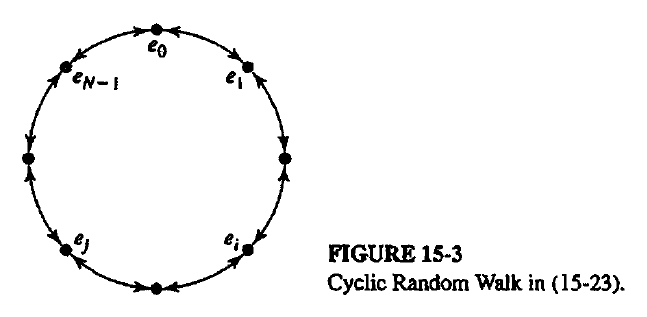
\includegraphics[height = 4cm]{figs/figure}
\end{center}

\end{frame}

\end{document}